\documentclass[a4paper]{article}

\usepackage[margin=1in]{geometry}
\usepackage[utf8]{inputenc}
\usepackage[T1]{fontenc}
\usepackage{mathrsfs}
\usepackage{textcomp}
\usepackage[french]{babel}
\usepackage{amsmath}
\usepackage{amssymb}
\usepackage{cancel}
\usepackage{frcursive}
\usepackage[inline]{asymptote}
\usepackage{tikz}
\usepackage[european,straightvoltages,europeanresistors]{circuitikz}
\usepackage{tikz-cd}
\usepackage{tkz-tab}
\usepackage[b]{esvect}
\usepackage[framemethod=TikZ]{mdframed}
\usepackage{centernot}
\usepackage{diagbox}
\usepackage{dsfont}
\usepackage{fancyhdr}
\usepackage{float}
\usepackage{graphicx}
\usepackage{listings}
\usepackage{multicol}
\usepackage{nicematrix}
\usepackage{pdflscape}
\usepackage{stmaryrd}
\usepackage{xfrac}
\usepackage{hep-math-font}
\usepackage{amsthm}
\usepackage{thmtools}
\usepackage{indentfirst}
\usepackage[framemethod=TikZ]{mdframed}
\usepackage{accents}
\usepackage{soulutf8}
\usepackage{mathtools}
\usepackage{bodegraph}
\usepackage{slashbox}
\usepackage{enumitem}
\usepackage{calligra}
\usepackage{cinzel}
\usepackage{BOONDOX-calo}

% Tikz
\usetikzlibrary{babel}
\usetikzlibrary{positioning}
\usetikzlibrary{calc}

% global settings
\frenchspacing
\reversemarginpar
\setuldepth{a}

%\everymath{\displaystyle}

\frenchbsetup{StandardLists=true}

\def\asydir{asy}

%\sisetup{exponent-product=\cdot,output-decimal-marker={,},separate-uncertainty,range-phrase=\;à\;,locale=FR}

\setlength{\parskip}{1em}

\theoremstyle{definition}

% Changing math
\let\emptyset\varnothing
\let\ge\geqslant
\let\le\leqslant
\let\preceq\preccurlyeq
\let\succeq\succcurlyeq
\let\ds\displaystyle
\let\ts\textstyle

\newcommand{\C}{\mathds{C}}
\newcommand{\R}{\mathds{R}}
\newcommand{\Z}{\mathds{Z}}
\newcommand{\N}{\mathds{N}}
\newcommand{\Q}{\mathds{Q}}

\renewcommand{\O}{\emptyset}

\newcommand\ubar[1]{\underaccent{\bar}{#1}}

\renewcommand\Re{\expandafter\mathfrak{Re}}
\renewcommand\Im{\expandafter\mathfrak{Im}}

\let\slantedpartial\partial
\DeclareRobustCommand{\partial}{\text{\rotatebox[origin=t]{20}{\scalebox{0.95}[1]{$\slantedpartial$}}}\hspace{-1pt}}

% merging two maths characters w/ \charfusion
\makeatletter
\def\moverlay{\mathpalette\mov@rlay}
\def\mov@rlay#1#2{\leavevmode\vtop{%
   \baselineskip\z@skip \lineskiplimit-\maxdimen
   \ialign{\hfil$\m@th#1##$\hfil\cr#2\crcr}}}
\newcommand{\charfusion}[3][\mathord]{
    #1{\ifx#1\mathop\vphantom{#2}\fi
        \mathpalette\mov@rlay{#2\cr#3}
      }
    \ifx#1\mathop\expandafter\displaylimits\fi}
\makeatother

% custom math commands
\newcommand{\T}{{\!\!\,\top}}
\newcommand{\avrt}[1]{\rotatebox{-90}{$#1$}}
\newcommand{\bigcupdot}{\charfusion[\mathop]{\bigcup}{\cdot}}
\newcommand{\cupdot}{\charfusion[\mathbin]{\cup}{\cdot}}
%\newcommand{\danger}{{\large\fontencoding{U}\fontfamily{futs}\selectfont\char 66\relax}\;}
\newcommand{\tendsto}[1]{\xrightarrow[#1]{}}
\newcommand{\vrt}[1]{\rotatebox{90}{$#1$}}
\newcommand{\tsup}[1]{\textsuperscript{\underline{#1}}}
\newcommand{\tsub}[1]{\textsubscript{#1}}

\renewcommand{\mod}[1]{~\left[ #1 \right]}
\renewcommand{\t}{{}^t\!}
\newcommand{\s}{\text{\calligra s}}

% custom units / constants
%\DeclareSIUnit{\litre}{\ell}
\let\hbar\hslash

% header / footer
\pagestyle{fancy}
\fancyhead{} \fancyfoot{}
\fancyfoot[C]{\thepage}

% fonts
\let\sc\scshape
\let\bf\bfseries
\let\it\itshape
\let\sl\slshape

% custom math operators
\let\th\relax
\let\det\relax
\DeclareMathOperator*{\codim}{codim}
\DeclareMathOperator*{\dom}{dom}
\DeclareMathOperator*{\gO}{O}
\DeclareMathOperator*{\po}{\text{\cursive o}}
\DeclareMathOperator*{\sgn}{sgn}
\DeclareMathOperator*{\simi}{\sim}
\DeclareMathOperator{\Arccos}{Arccos}
\DeclareMathOperator{\Arcsin}{Arcsin}
\DeclareMathOperator{\Arctan}{Arctan}
\DeclareMathOperator{\Argsh}{Argsh}
\DeclareMathOperator{\Arg}{Arg}
\DeclareMathOperator{\Aut}{Aut}
\DeclareMathOperator{\Card}{Card}
\DeclareMathOperator{\Cl}{\mathcal{C}\!\ell}
\DeclareMathOperator{\Cov}{Cov}
\DeclareMathOperator{\Ker}{Ker}
\DeclareMathOperator{\Mat}{Mat}
\DeclareMathOperator{\PGCD}{PGCD}
\DeclareMathOperator{\PPCM}{PPCM}
\DeclareMathOperator{\Supp}{Supp}
\DeclareMathOperator{\Vect}{Vect}
\DeclareMathOperator{\argmax}{argmax}
\DeclareMathOperator{\argmin}{argmin}
\DeclareMathOperator{\ch}{ch}
\DeclareMathOperator{\com}{com}
\DeclareMathOperator{\cotan}{cotan}
\DeclareMathOperator{\det}{det}
\DeclareMathOperator{\id}{id}
\DeclareMathOperator{\rg}{rg}
\DeclareMathOperator{\rk}{rk}
\DeclareMathOperator{\sh}{sh}
\DeclareMathOperator{\th}{th}
\DeclareMathOperator{\tr}{tr}

% colors and page style
\definecolor{truewhite}{HTML}{ffffff}
\definecolor{white}{HTML}{faf4ed}
\definecolor{trueblack}{HTML}{000000}
\definecolor{black}{HTML}{575279}
\definecolor{mauve}{HTML}{907aa9}
\definecolor{blue}{HTML}{286983}
\definecolor{red}{HTML}{d7827e}
\definecolor{yellow}{HTML}{ea9d34}
\definecolor{gray}{HTML}{9893a5}
\definecolor{grey}{HTML}{9893a5}
\definecolor{green}{HTML}{a0d971}

\pagecolor{white}
\color{black}

\begin{asydef}
	settings.prc = false;
	settings.render=0;

	white = rgb("faf4ed");
	black = rgb("575279");
	blue = rgb("286983");
	red = rgb("d7827e");
	yellow = rgb("f6c177");
	orange = rgb("ea9d34");
	gray = rgb("9893a5");
	grey = rgb("9893a5");
	deepcyan = rgb("56949f");
	pink = rgb("b4637a");
	magenta = rgb("eb6f92");
	green = rgb("a0d971");
	purple = rgb("907aa9");

	defaultpen(black + fontsize(8pt));

	import three;
	currentlight = nolight;
\end{asydef}

% theorems, proofs, ...

\mdfsetup{skipabove=1em,skipbelow=1em, innertopmargin=6pt, innerbottommargin=6pt,}

\declaretheoremstyle[
	headfont=\normalfont\itshape,
	numbered=no,
	postheadspace=\newline,
	headpunct={:},
	qed=\qedsymbol]{demstyle}

\declaretheorem[style=demstyle, name=Démonstration]{dem}

\newcommand\veczero{\kern-1.2pt\vec{\kern1.2pt 0}} % \vec{0} looks weird since the `0' isn't italicized

\makeatletter
\renewcommand{\title}[2]{
	\AtBeginDocument{
		\begin{titlepage}
			\begin{center}
				\vspace{10cm}
				{\Large \sc Chapitre #1}\\
				\vspace{1cm}
				{\Huge \calligra #2}\\
				\vfill
				Hugo {\sc Salou} MPI${}^{\star}$\\
				{\small Dernière mise à jour le \@date }
			\end{center}
		\end{titlepage}
	}
}

\newcommand{\titletp}[4]{
	\AtBeginDocument{
		\begin{titlepage}
			\begin{center}
				\vspace{10cm}
				{\Large \sc tp #1}\\
				\vspace{1cm}
				{\Huge \textsc{\textit{#2}}}\\
				\vfill
				{#3}\textit{MPI}${}^{\star}$\\
			\end{center}
		\end{titlepage}
	}
	\fancyfoot{}\fancyhead{}
	\fancyfoot[R]{#4 \textit{MPI}${}^{\star}$}
	\fancyhead[C]{{\sc tp #1} : #2}
	\fancyhead[R]{\thepage}
}

\newcommand{\titletd}[2]{
	\AtBeginDocument{
		\begin{titlepage}
			\begin{center}
				\vspace{10cm}
				{\Large \sc td #1}\\
				\vspace{1cm}
				{\Huge \calligra #2}\\
				\vfill
				Hugo {\sc Salou} MPI${}^{\star}$\\
				{\small Dernière mise à jour le \@date }
			\end{center}
		\end{titlepage}
	}
}
\makeatother

\newcommand{\sign}{
	\null
	\vfill
	\begin{center}
		{
			\fontfamily{ccr}\selectfont
			\textit{\textbf{\.{\"i}}}
		}
	\end{center}
	\vfill
	\null
}

\renewcommand{\thefootnote}{\emph{\alph{footnote}}}

% figure support
\usepackage{import}
\usepackage{xifthen}
\pdfminorversion=7
\usepackage{pdfpages}
\usepackage{transparent}
\newcommand{\incfig}[1]{%
	\def\svgwidth{\columnwidth}
	\import{./figures/}{#1.pdf_tex}
}

\pdfsuppresswarningpagegroup=1
\ctikzset{tripoles/european not symbol=circle}

\newcommand{\missingpart}{{\large\color{red} Il manque quelque chose ici\ldots}}


\pagecolor{truewhite}
\color{trueblack}

\titletp{ts 1}{Rappels sur quelques appareils d'utilisation courante}
{
	\begin{tabular}{c}
		Hugo {\sc Salou}\/\\
		Alan {\sc Le Brech}\/\\
		Nicolas {\sc Vincent}\/
	\end{tabular}
}

\begin{document}
	\begin{multicols}{2}
		L'objectif de ce {\sc Tp}\/ est de réutiliser des appareils électriques utilisés l'année dernière en {\it MP2I}\/ (multimètre, oscilloscope, {\sc Gbf}, dipôles$,\ldots$) afin de mesurer des grandeurs communes en électricité.

		La notation ``$\triangleq$\/'' sera utilisée pour la définitions d'une grandeur ; tandis que la notation ``$\circeq$\/'' sera utilisée pour les applications numériques et valeurs mesurées.

		\section{Prise en main des appareils ({\sc Gbf}, oscilloscope, multimètre}

		On génère à l'aide du {\sc Gbf}\/ un signal de fréquence $f = 1\:\mathrm{kHz}$, d'amplitude $2\:\mathrm{V}$\/ et de valeur moyenne $0{,}5\:\mathrm{V}$.
		Ces valeurs ont été obtenues à l'aide d'un oscilloscope mais nous re-mesurons ces valeurs à l'aide du multimètre. On obtient une fréquence $f \circeq 1{,}156\:\mathrm{kHz}$, une valeur moyenne $\langle s \rangle \circeq 0{,}600\:\mathrm{V}$, une valeur efficace de $1{,}44\:\mathrm{V}$\/ et une valeur efficace vraie de $1{,}55\:\mathrm{V}$. Les valeurs mesurées correspondent environ à celle demandées (une étude des incertitudes serait nécessaire pour savoir d'où viennent ces imprécisions) ; en effet, la valeur efficace théorique de ce signal serai de $2\:\mathrm{V} / \sqrt{2} \cong 1{,}41\:\mathrm{V}$.

		On vérifie maintenant la relation donnée dans le sujet : $S^2 = S_\mathrm{a}^2 + \langle s(t)\rangle^2$\/ où $S_\mathrm{a}$\/ est la valeur efficace et $S$\/ la valeur efficace vraie. On a \[
			\langle s(t)\rangle^2 \circeq 0{,}360\:\mathrm{V^2} \quad
			S_\mathrm{a}^2 \circeq 2{,}07\:\mathrm{V^2} \quad
			S^2 \circeq 2{,}40\:\mathrm{V^2}
		\]
		et, en calculant $S_\mathrm{a}^2 + \langle s(t)\rangle^2 \circeq 2{,}43\:\mathrm{V}$\/ ; la relation est donc vérifiée.

		La {\sc Figure 1}\/ représente le signal sinusoïdal obtenu à l'oscilloscope (tension $s(t)$\/ en fonction du temps $t$).
	\end{multicols}

	\begin{figure}[H]
		\centering
		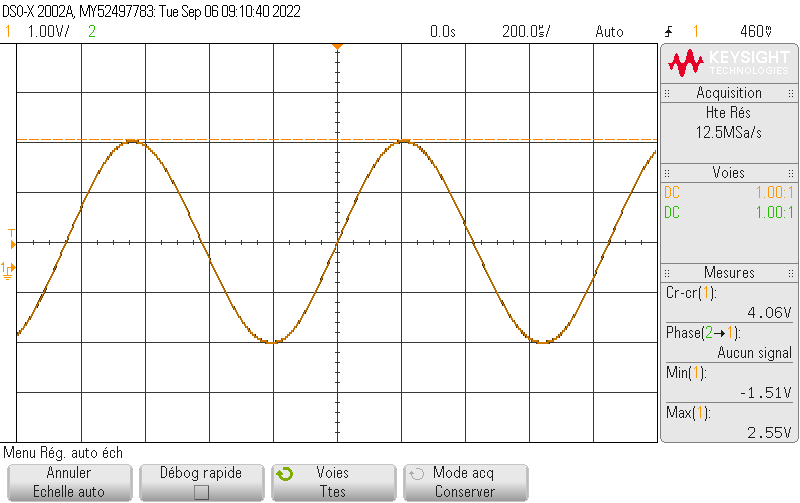
\includegraphics[scale=0.4]{figures/signal1.png}
		\caption{Signal sinusoïdal à l'oscilloscope}
	\end{figure}
	
	\begin{multicols}{2}
		On génère ensuite un autre signal créneau de même fréquence $f = 1\: \mathrm{kHz}$, de même amplitude $2\:\mathrm{V}$\/ et de même valeur moyenne $0{,}5\:\mathrm{V}$. En re-mesurant au multimètre les caractéristiques de ce signal, on obtient une même fréquence ($f \circeq 1{,}180\:\mathrm{kHz}$), une même valeur moyenne ($\langle s'(t) \rangle \circeq 0{,}480\:\mathrm{V}$) mais les valeurs efficaces changent : la valeur efficace est de $S'_\mathrm{a} \circeq 2{,}01\:\mathrm{V}$\/ et la valeur efficace vraie est de $S' \circeq 2{,}07\:\mathrm{V}$. La relation est également vérifiée : \[
			\begin{array}{cccccr}
				{S'}^2 &=& {S'_\mathrm{a}}^2 &+& \langle s'(t) \rangle^2\\[2mm]
				\vrt\circeq&&\vrt\circeq&&\vrt\circeq\\[2mm]
				4{,}29\:\mathrm{V^2}&\cong&4{,}04\:\mathrm{V^2}&+&0{,}230\:\mathrm{V}^2 &\:\circeq\:4{,}27\:\mathrm{V}^2.
			\end{array}
		\]

		\section{Montage RC en régime sinusoïdal}

		On réalise le montage RC (comme montré dans la {\sc Figure 2}), avec une résistance de $R = 1{,}\:\mathrm{k\Omega}$, un condensateur de $C = 100\:\mathrm{nF}$, et un signal de fréquence $f = 2\:\mathrm{kHz}$\/ d'amplitude $2\:\mathrm{V}$.

		On vérifie ces valeurs à l'ohmmètre et à l'impédancemètre ; on obtient des valeurs proches de celles demandées, à savoir : $R \circeq 0{,}993\:\mathrm{k\Omega}$\/ et $L \circeq 99{,}9\:\mathrm{nF}$.
	\end{multicols}

	\begin{figure}[H]
		\centering
		\begin{circuitikz}
			\draw (0,0) to[sinusoidal voltage source,v=$v_\mathrm{e}$] (0, 2) to[R=$R$] (4, 2) to[C=$C$, v=$v_\mathrm{s}$] (4, 0) -- (0, 0);
		\end{circuitikz}
		\caption{Circuit du montage RC}
	\end{figure}

	\begin{multicols}{2}
		Le déphasage $\mathrm{\Delta}\varphi$\/ entre les signaux $v_\text{e}$\/ et $v_\text{s}$\/ est défini comme \[
			\mathrm{\Delta}\varphi \triangleq \frac{2\pi\,\mathrm{\Delta}t}{T}
		\] où $T$\/ est la période du signal d'entrée, i.e.\ $T = \frac{1}{f}$, et $\mathrm{\Delta}t$\/ est l'intervalle de temps entre le maximum du signal $v_\text{e} $\/ et celui du signal $v_\text{s}$.

		On mesure $\mathrm{\Delta}t \circeq -71\:\mathrm{\mu s}$, et on en déduit que le signal d'entrée est en avance. On calcule $\mathrm{\Delta}\varphi = 2\pi\,\mathrm{\Delta}t\,f \circeq -0{,}89\:\mathrm{rad}$. On mesure également à l'oscilloscope le déphasage et on obtient une valeur proche : $0{,}87\:\mathrm{rad}$.
		On peut également vérifier avec le diagramme de {\sc Bode}\/ : avec lecture graphique, on a, pour $f = 2\:\mathrm{kHz}$, $\mathrm{\Delta}\varphi = 50^\circ = 0{,}87\:\mathrm{rad}$.

		On mesure, à l'aide de l'oscilloscope, la tension $v_\text{e}$\/ et $v_\text{s}$\/ puis on calcule le quotient $G$\/ des deux : \[
			\left.
				\begin{array}{r}
					v_\text{s} \circeq 4{,}4\:\mathrm{V}\\
					v_\text{e} \circeq 7{,}1\:\mathrm{V}\\
				\end{array}
			\right\}\quad\text{d'où}\quad G \circeq 0{,}62
		.\] On peut également en déduire le gain en dB du montage RC : $G_\text{dB} \triangleq 20\log G \circeq -4{,}2\:\mathrm{dB}$. Ce gain correspond au gain indiqué dans le diagramme de {\sc Bode}.

		On analyse le comportement de filtre : il s'agit d'un filtre passe-bas.
		On change la fréquence du signal d'entrée. On s'attend à ce que, pour une fréquence basse, le gain soit environ à 1 ; et que, pour une fréquence haute, le gain soit proche de 0 de telle sorte à ce que les signaux à hautes fréquences soient filtrés.
		On vérifie expérimentalement ce comportement : pour $f \circeq 113\:\mathrm{Hz}$, on a $\smash{G \triangleq \sfrac{v_\text{s}}{v_\text{e}} \circeq \sfrac{20{,}3\:\mathrm{V}}{20{,}3\:\mathrm{V}} \circeq 1}$ ; et, pour $\smash{f \circeq 31{,}1\:\mathrm{kHz}}$, on a $\smash{G \circeq \sfrac{1{,}05\:\mathrm{V}}{19{,}6\:\mathrm{V}} \circeq 0{,}05}$.
		Le caractère passe-bas du montage RC est bien vérifié.

		On cherche maintenant la fréquence de coupure à $-3\:\mathrm{dB}$\/ : on sait premièrement que le gain maximal est 1 et correspond aux petites fréquences. On cherche donc le gain (pas en $\mathrm{dB}$) associé à la fréquence de coupure :
		on sait que $G_\text{coup.} \triangleq \sfrac{1}{\sqrt{2}}$, et, comme le signal est à environ $v_\text{e} = 20\:\mathrm{V}$\/ constamment, on cherche la fréquence de coupure $f_\text{coup.}$\/ quand la tension $v_\text{s} $\/ sera à environ $\smash{v_\text{s,coup.} \circeq 20\:\mathrm{V} / \sqrt{2} \circeq 14\:\mathrm{V}}$.
		On parcourt les fréquences et on trouve une fréquence $f_\text{coup.} \circeq 1{,}65\:\mathrm{kHz}$.
		On vérifie sur le diagramme de {\sc Bode}, et la fréquence de coupure correspond.

		\section{Circuit linéaire en régime transitoire~: les régimes libres d'un circuit du second ordre RLC}

		On s'intéresse maintenant au montage RLC : la {\sc Figure 3}\/ représente le schéma du circuit électrique RLC. On sait, tout d'abord, que le circuit RLC a pour équation différentielle celle d'un oscillateur amorti : \[
			\frac{\mathrm{d}^2s}{\mathrm{d}t^2} + \frac{\omega_0}{Q}\frac{\mathrm{d}s}{\mathrm{d}t} + \omega_0^2 s = 0
		.\] Les expressions de $\omega_0$\/ et de $Q$\/ sont connues : on a \[
			\omega_0 = \frac{1}{\sqrt{LC}}\quad\text{et}\quad Q = \frac{1}{R}\sqrt{\frac{L}{C}}
		.\]
		Le résultat dépend de la valeur de $Q$\/ utilisée : avec $0 < Q < \sfrac12$, on a le régime apériodique ; avec $Q = \sfrac12$, on a le régime critique ; et, avec $Q > \sfrac12$, on a le régime pseudo-périodique.
		La {\sc Figure 4}\/ montre l'allure des différents régimes.
	\end{multicols}

	\begin{minipage}{0.5\textwidth}
		\begin{figure}[H]
			\centering
			\begin{circuitikz}
				\draw (0,0) to[american, isource, l=$E$] (0, 2);
				\draw[-o] (0, 2) -- (1.6, 2);
				\draw (0,0) -- (2, 0) to[C=$C$] (2, 1.6);
				\draw[-*] (2, 1.5) -- (2, 1.6);
				\draw (2, 1.6) -- (1.6, 2);
				\node at (1.6, 2.3) {\llap{$1$}};
				\node at (2.4, 2.3) {\llap{$2$}};
				\draw[o-] (2.4, 2) -- (4, 2);
				\draw (4,2) to[american,cute inductors,L=$L$] (4, 0) to[R=$R$,v=$v_\text{s}$] (2, 0);
			\end{circuitikz}
			\caption{Circuit du montage RLC}
		\end{figure}
	\end{minipage}
	\begin{minipage}{0.5\textwidth}
		\begin{figure}[H]
			\centering
			\begin{asy}
				import graph; 

				size(7cm);
				draw((-0.5,0)--(15, 0), Arrow(TeXHead));
				draw((0,-3)--(0, 5), Arrow(TeXHead));

				real f(real x) {return sin(1.5x) * exp(-x/5) * 5;}
				real g(real x) {return x * exp(-x/2) * 5;}

				real h(real x) {return 15 * (exp(-x/2) - exp(-x));}

				draw(graph(f, 0, 15, 200), magenta);
				draw(graph(g, 0, 15, 200), deepcyan);
				draw(graph(h, 0, 15, 200), green);

				label("$Q > \sfrac12$", (3,f(3)), magenta, align=SW);
				label("$Q = \sfrac12$", (3.5,g(3.5)), deepcyan, align=NE);
				label("$Q < \sfrac12$", (2,h(2)+0.5), green, align=N);
			\end{asy}
			\caption{Les différents régimes du circuit RLC}
		\end{figure}
	\end{minipage}

	\bigskip

	\begin{multicols}{2}
		Nous n'avons pas pu observer tous les régimes du circuit RLC mais uniquement celui du régime pseudo-périodique, autrement dit, pour $Q > \sfrac{1}{2}$.
		La {\sc Figure~5}\/ représente la mesure à l'oscilloscope de la tension $v_\text{s}$\/ en fonction du temps.

		Le résultat obtenu étant très proche de l'allure du régime pseudo-périodique théorique, on en déduit que le modèle du circuit RLC est valide.
	\end{multicols}

	\bigskip

	\begin{figure}[H]
		\centering
		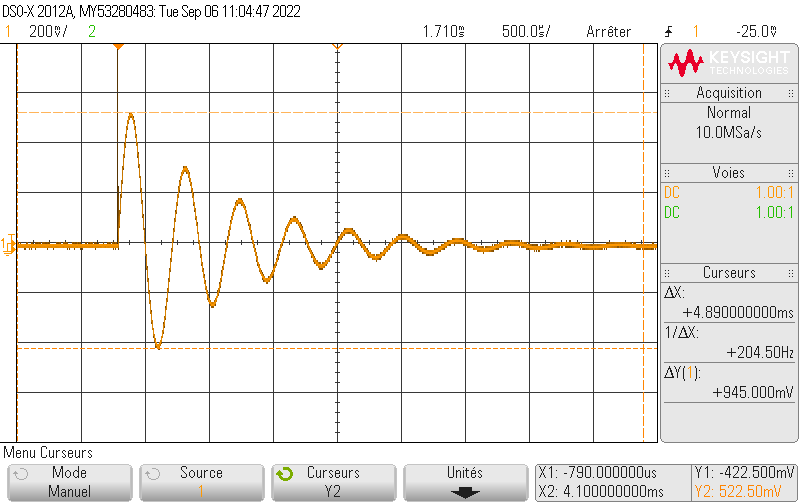
\includegraphics[scale=0.4]{figures/signal2.png}
		\caption{Réponse pseudo-périodique du circuit RLC}
	\end{figure}

	\sign
\end{document}
